\section{Geoinformationssysteme}
\label{sec:GIS}
% Nach \cite{de_lange_geoinformatik_2020} ist ein Geoinformationssystem (GIS) ein Informationssystem, das sich auf Modellierung und digitale Abbildungen von Geoobjekte der realen Welt konzentriert. Dieses System erfasst, verarbeitet, speichert, visualisieret und wertet raumbezogene Informationen aus. Dies erfordert spezielle Werkzeuge und Funktionen. \\

``Ein Geoinformationssystem ist ein rechnergestütztes System, das aus Hardware, Software, Daten und den Anwendungen besteht. Mit ihm können raumbezogene Daten digital erfasst, gespeichert, verwaltet, aktualisiert, analysiert und modelliert sowie alphanumerisch und graphisch präsentiert werden.'' \citep[S. ~375]{de_lange_geoinformatik_2020} GIS konzentriert sich auf Modellierung und digitale Abbildungen von Geoobjekten der realen Welt. Es besteht aus Hardware, Software, Daten und Anwendern. zur Visualisierung von Geodaten werden solche Dienste wie GoogleMaps, OpenStreetMap oder Basemap.de angesporchen. \\


Die Abbildung 2.5 illustriert das Konzept, wie Daten in einem GIS durch die Darstellung verschiedener Schichten organisiert werden, um realen Welt zu digitalisieren. Sie bildet ab, wie die physische Welt in GIS-Datenbank strukturiert wird, um eine Vielzahl von Analysen und Funktionen zu unterstützen. 
\begin{figure}[ht]
  \centering
  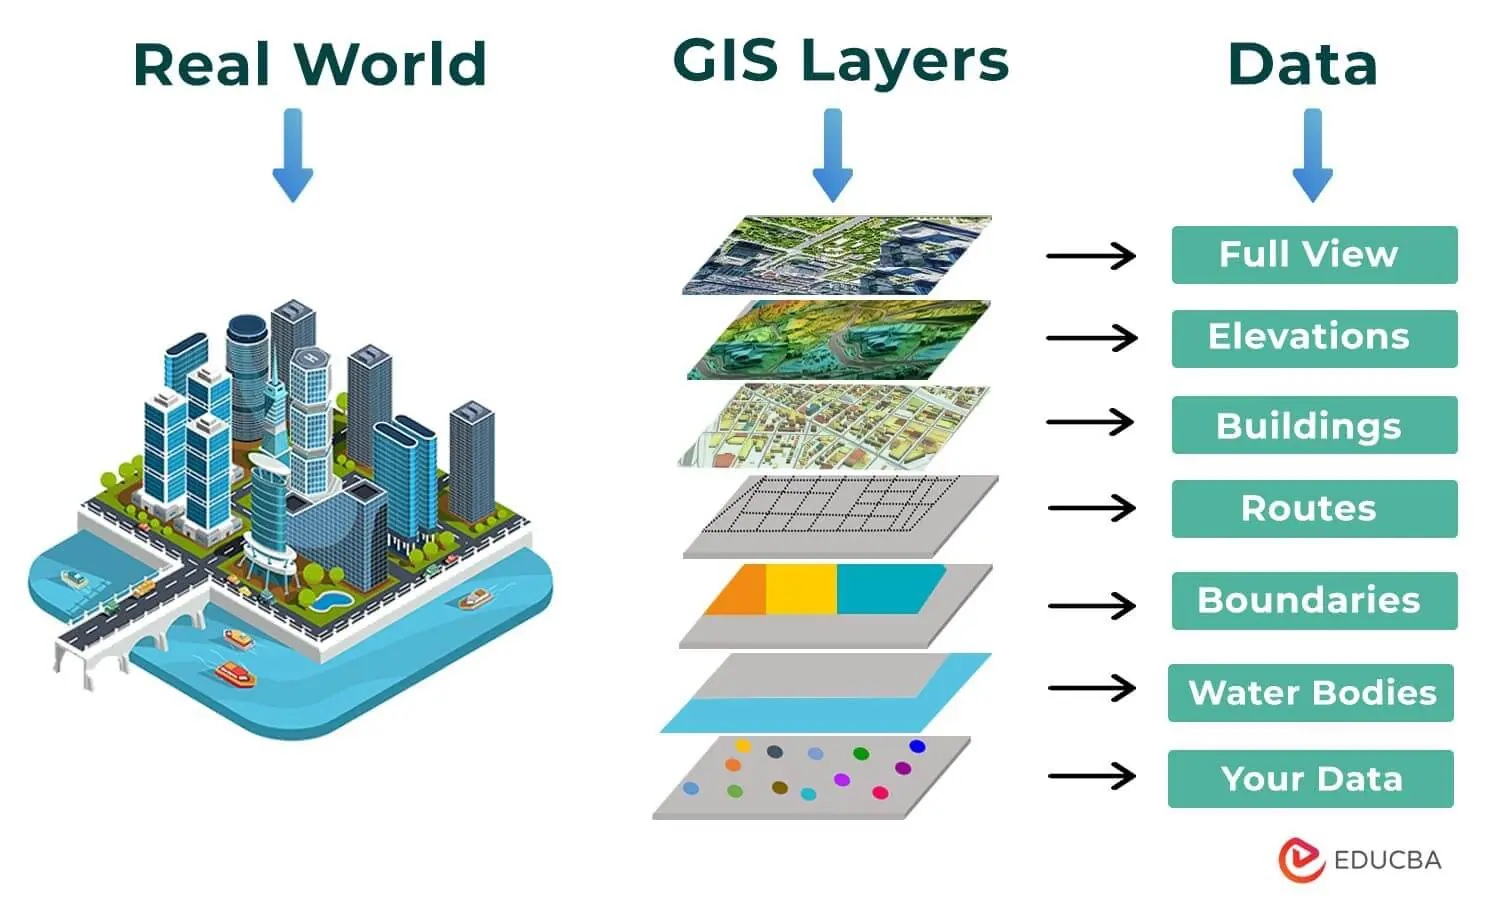
\includegraphics[width=\linewidth]{images/gis.jpg}
  \caption{Konzept der Datenorganisation in einem GIS \citep{gis_bild}}
  \label{fig:meineabbildung}
\end{figure}

Moderne GIS sind vielseitig und bieten eine breite Palette von Funktionen. Hier sind neben Visualisierung weitere Funktionsmöglichkeiten von GIS:
\begin{itemize}
    \item Datenerfassung und -bearbeitung.
    \item Ermittlung von Standorten, Mustern und Beziehungen zwischen verschiedenen Geoobjekten.
    \item Analysieren von Distanzen, Flächen und räumlichen Überlappungen
    \item Sammeln, speichern und verwalten großer Mengen Geodaten.
    \item Integration und Verwaltung verschiedener Datenformate und -quellen.
    \item Erstellung von Routen.
    \item Überwachung und Analyse von Umweltveränderungen und -auswirkungen.
\end{itemize}

In gewerblichen Bereichen dominieren kommerzielle Geoinformationssystem wie ArcGIS und Map3D. Die bekanntesten Open-Source-GIS sind QGIS und GRASS GIS. Es gibt zahlreiche GIS-Werkzeuge wie Openlayers, Leaflet. Online-GIS sind beispielsweise Google Maps, OpenStreetMap. Und die webbasierte GIS sind Server-Software, die auf Geodaten spezialisierte Geodienste zur Verfügung gestellt wie MapServer, Geoserver.\\

Im Rahmen dieser Bachelorarbeit werde ich für das Showcase einen GIS-Modul nach die Anforderungen (Kapitel 3) der Telekom MMS GmbH konzepieren und entwickeln, um eine Karte inklusive Daten von Schulen in einem Schulanmeldung Formular zu visualisieren. Für die Implementierung von GIS wird eine leistungsstarke JavaScript-basierte Bibliothek Openlayers als Werkzeug genutzt. Die wird in nächsten Abschnitt näher erklärt.


